% 최종 축약본. chapter4.md와 같은 본문에서 생성.
\subsection{질문 조건에 따른 성능 차이}
\label{sec:ch4_subgroups}

Jev의 근거 F1은 2·3-hop 질문에서 높았고, 1-hop에서는 소폭 낮았다(그림~\ref{fig:ch4_hop_f1}). hop은 평가 자료가 부여한 추론 단계 구분이며 실제 정답 근거 개수와는 다르다. 1-hop 57문항은 CE 78.07점, Jev 76.90점이었고, 2-hop 127문항은 53.33점과 57.24점, 3-hop 42문항은 47.91점과 54.83점이었다.

\begin{figure}[htbp]
\centering
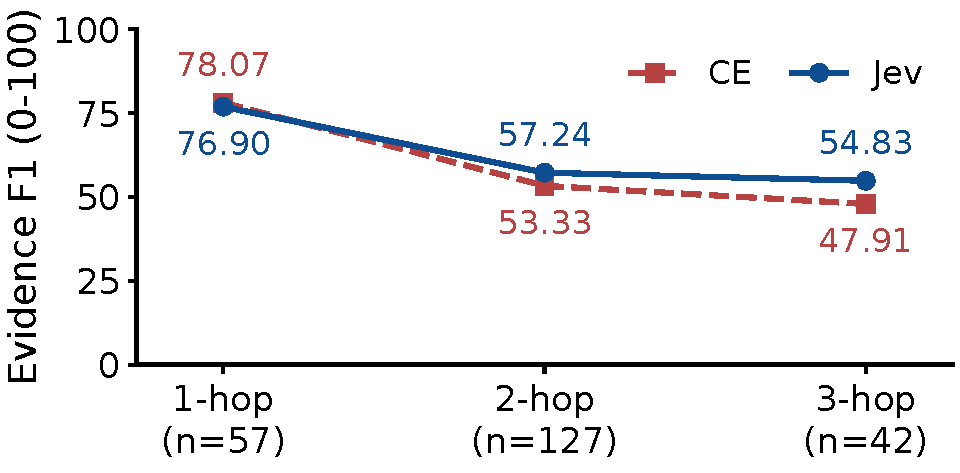
\includegraphics[width=\linewidth]{research/chapter4/figures/hop_f1.pdf}
\caption{추론 단계별 근거 F1. 집단별 신뢰구간은 산출하지 않았다.}
\label{fig:ch4_hop_f1}
\end{figure}

이는 관측 평균의 차이로, 추론 단계에 따라 교체 효과가 달라지는지는 별도로 검정하지 않았다. 특히 3-hop의 완전 회수는 두 조건 모두 1문항(2.38\%)이었다. F1이 높아져도 모든 근거를 확보하는 문제는 남았다.

정답 근거를 검색 자료에서 찾을 수 있는지에 따라서도 차이가 컸다. 고유 정답 근거 386개 중 27개는 자료에서 동일 문자열을 찾을 수 없었다. 모든 근거가 대응된 197문항의 F1은 CE 64.12점, Jev 67.21점이었고, 불일치가 있는 29문항은 20.80점과 24.71점이었다. 후자의 낮은 점수에는 검색 성능뿐 아니라 자료의 제약도 반영된다. 문항별로는 Jev 개선 32개, 동일 177개, CE 우세 17개로, 전체 평균의 개선은 일부 질문의 변화에서 발생하였다. 질문들이 출처나 정답 근거를 공유할 수 있으므로, 이 개수를 서로 독립적인 시행의 성공률로 해석하지 않았다.
